\documentclass{beamer}
\usepackage{beamerthemesplit}
\usepackage{graphics}
\usepackage{pstricks}
\usepackage[T2A]{fontenc}			% кодировка
\usepackage[utf8]{inputenc}			% кодировка исходного текста
\usepackage[english,russian]{babel}	% локализация и переносы
%grek
\usepackage{ tipa }
\usepackage{ amssymb }

\usepackage{caption, subcaption}
\usepackage{wasysym}
%\usepackage{enumitem}
\graphicspath{ {img/} }


\title{Кафедра нанометрологии и наноматериалов}
\author{Михаил Соловьянов}


\begin{document}


\frame{
   \begin{center}
    \huge{Создание энергоэффективных блоков сегнетоэлектрической памяти для нейроморфных приложений}\\
    \vspace{24pt}
    \Large{Научный руководитель: Дмитрий Владимирович Негров}\\
    \vspace{14pt}
    \Large{Соловьянов Михаил Михайлович}\\
    \vspace{24pt}
    \large{\today}
  \end{center}
}






\frame{\frametitle{Постановка задачи}
 \begin{center}
  \begin{enumerate}
   \item Разработать тестовый прототип FRAM памяти на новом сверхтонком слое сегнетоэлектрика, включающий в себя так же цифровой контроллер памяти и способный измерять остаточную поляризацию.
   
   \item Подготовить layout на базе существующей технологии для создания устройства. 
  \end{enumerate} %на самом деле задач было больше, но они не уместились на слайд!
 \end{center}
}







\frame{\frametitle{Сегнетоэлектрик из HfO2-ZnO2}
 \begin{center} 
 \begin{figure}
 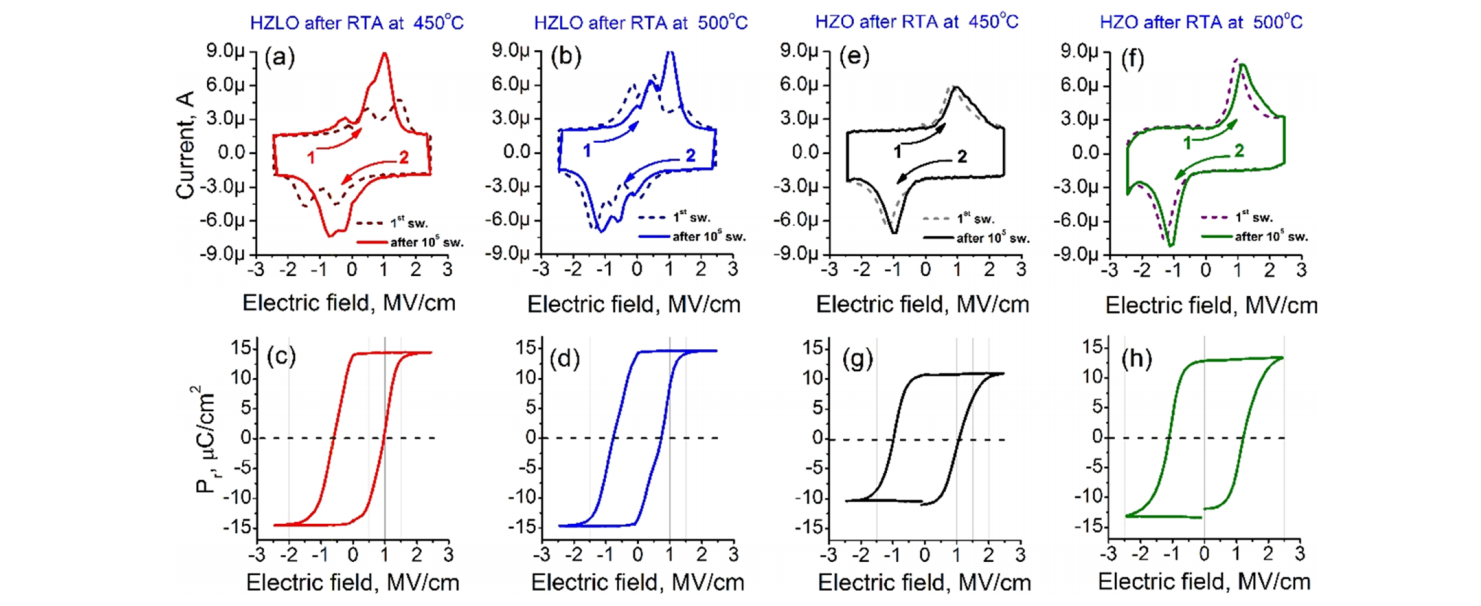
\includegraphics[width=0.90\textwidth]{graph0.png}
 \caption{Графики Поляризации от внешнего поля и ток через элемент при переполяризации, полученные в лабораториях ЦКП в 2016 году }
 \end{figure}

 \end{center}
}

%$Hf_{0.5}Zr_{0.5}O_2$
























\frame{\frametitle{Построение модели сегнетоэлектрика. Теория Ландау О фазовых переходах. }
 \begin{center}

  \begin{equation}\label{fermi}
   \mathcal{F} = \frac{1}{2}\alpha \vec{P}^2 + \frac{1}{4}\beta \vec{P}^4 - \vec{E}\vec{P}
  \end{equation}
   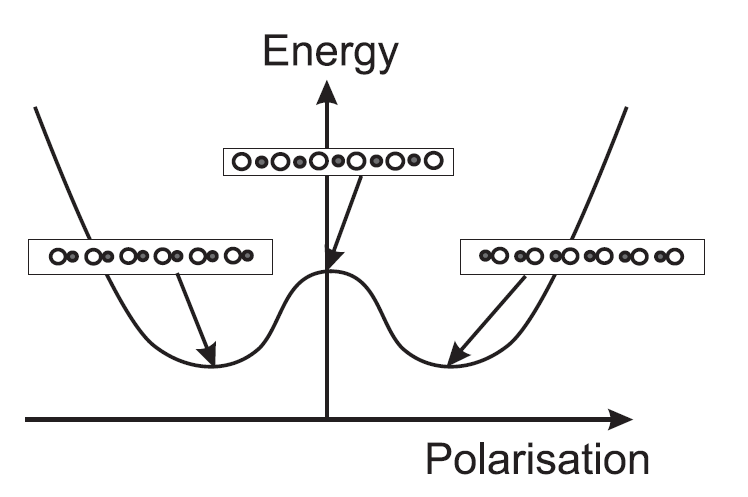
\includegraphics[width=0.5\textwidth]{F(P).png}%
	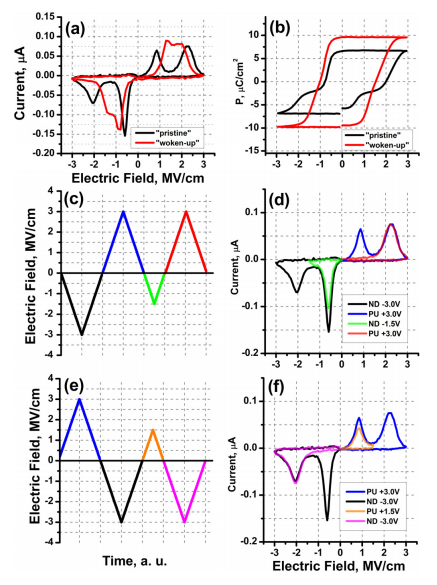
\includegraphics[width=0.5\textwidth]{Hyst.png}
	  Дифференцируя выражение \eqref{fermi} получаем:
  \begin{equation}\label{dfermi}
  \frac{\partial \mathcal{F}}{\partial P }  = \alpha P + \beta P^3 - E
  \end{equation}
 \end{center}
}









\frame{
  \begin{center}
  
	 \begin{equation}\label{Rfermi}
		 \frac{\partial  \mathcal{F} }{\partial P} = - R  \frac{\partial  P }{\partial t}  
 	 \end{equation}    
 	$$\alpha = 3\sqrt{3E_c/(8{P_0}^3)}$$
	$$ \beta = -3\sqrt{3E_c/(4P_0)}$$
	%  Приравнивая выражение  \eqref{dfermi} к \eqref{Rfermi} получаем :
  
  \begin{equation}
  -R \dot{\vec{P}}  = \alpha \vec{P} + \beta \vec{P}^3 - \vec{E}
  \end{equation}
  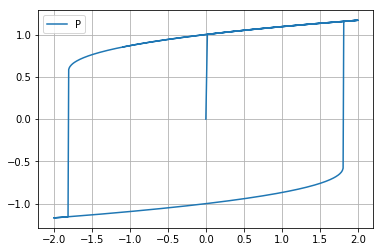
\includegraphics[width=0.6\textwidth]{Python-sym.png}
  \end{center}
}










\frame{\frametitle{Строение Ferroelectric Random Access Memory (FRAM) }
 \begin{center}

 \begin{figure}
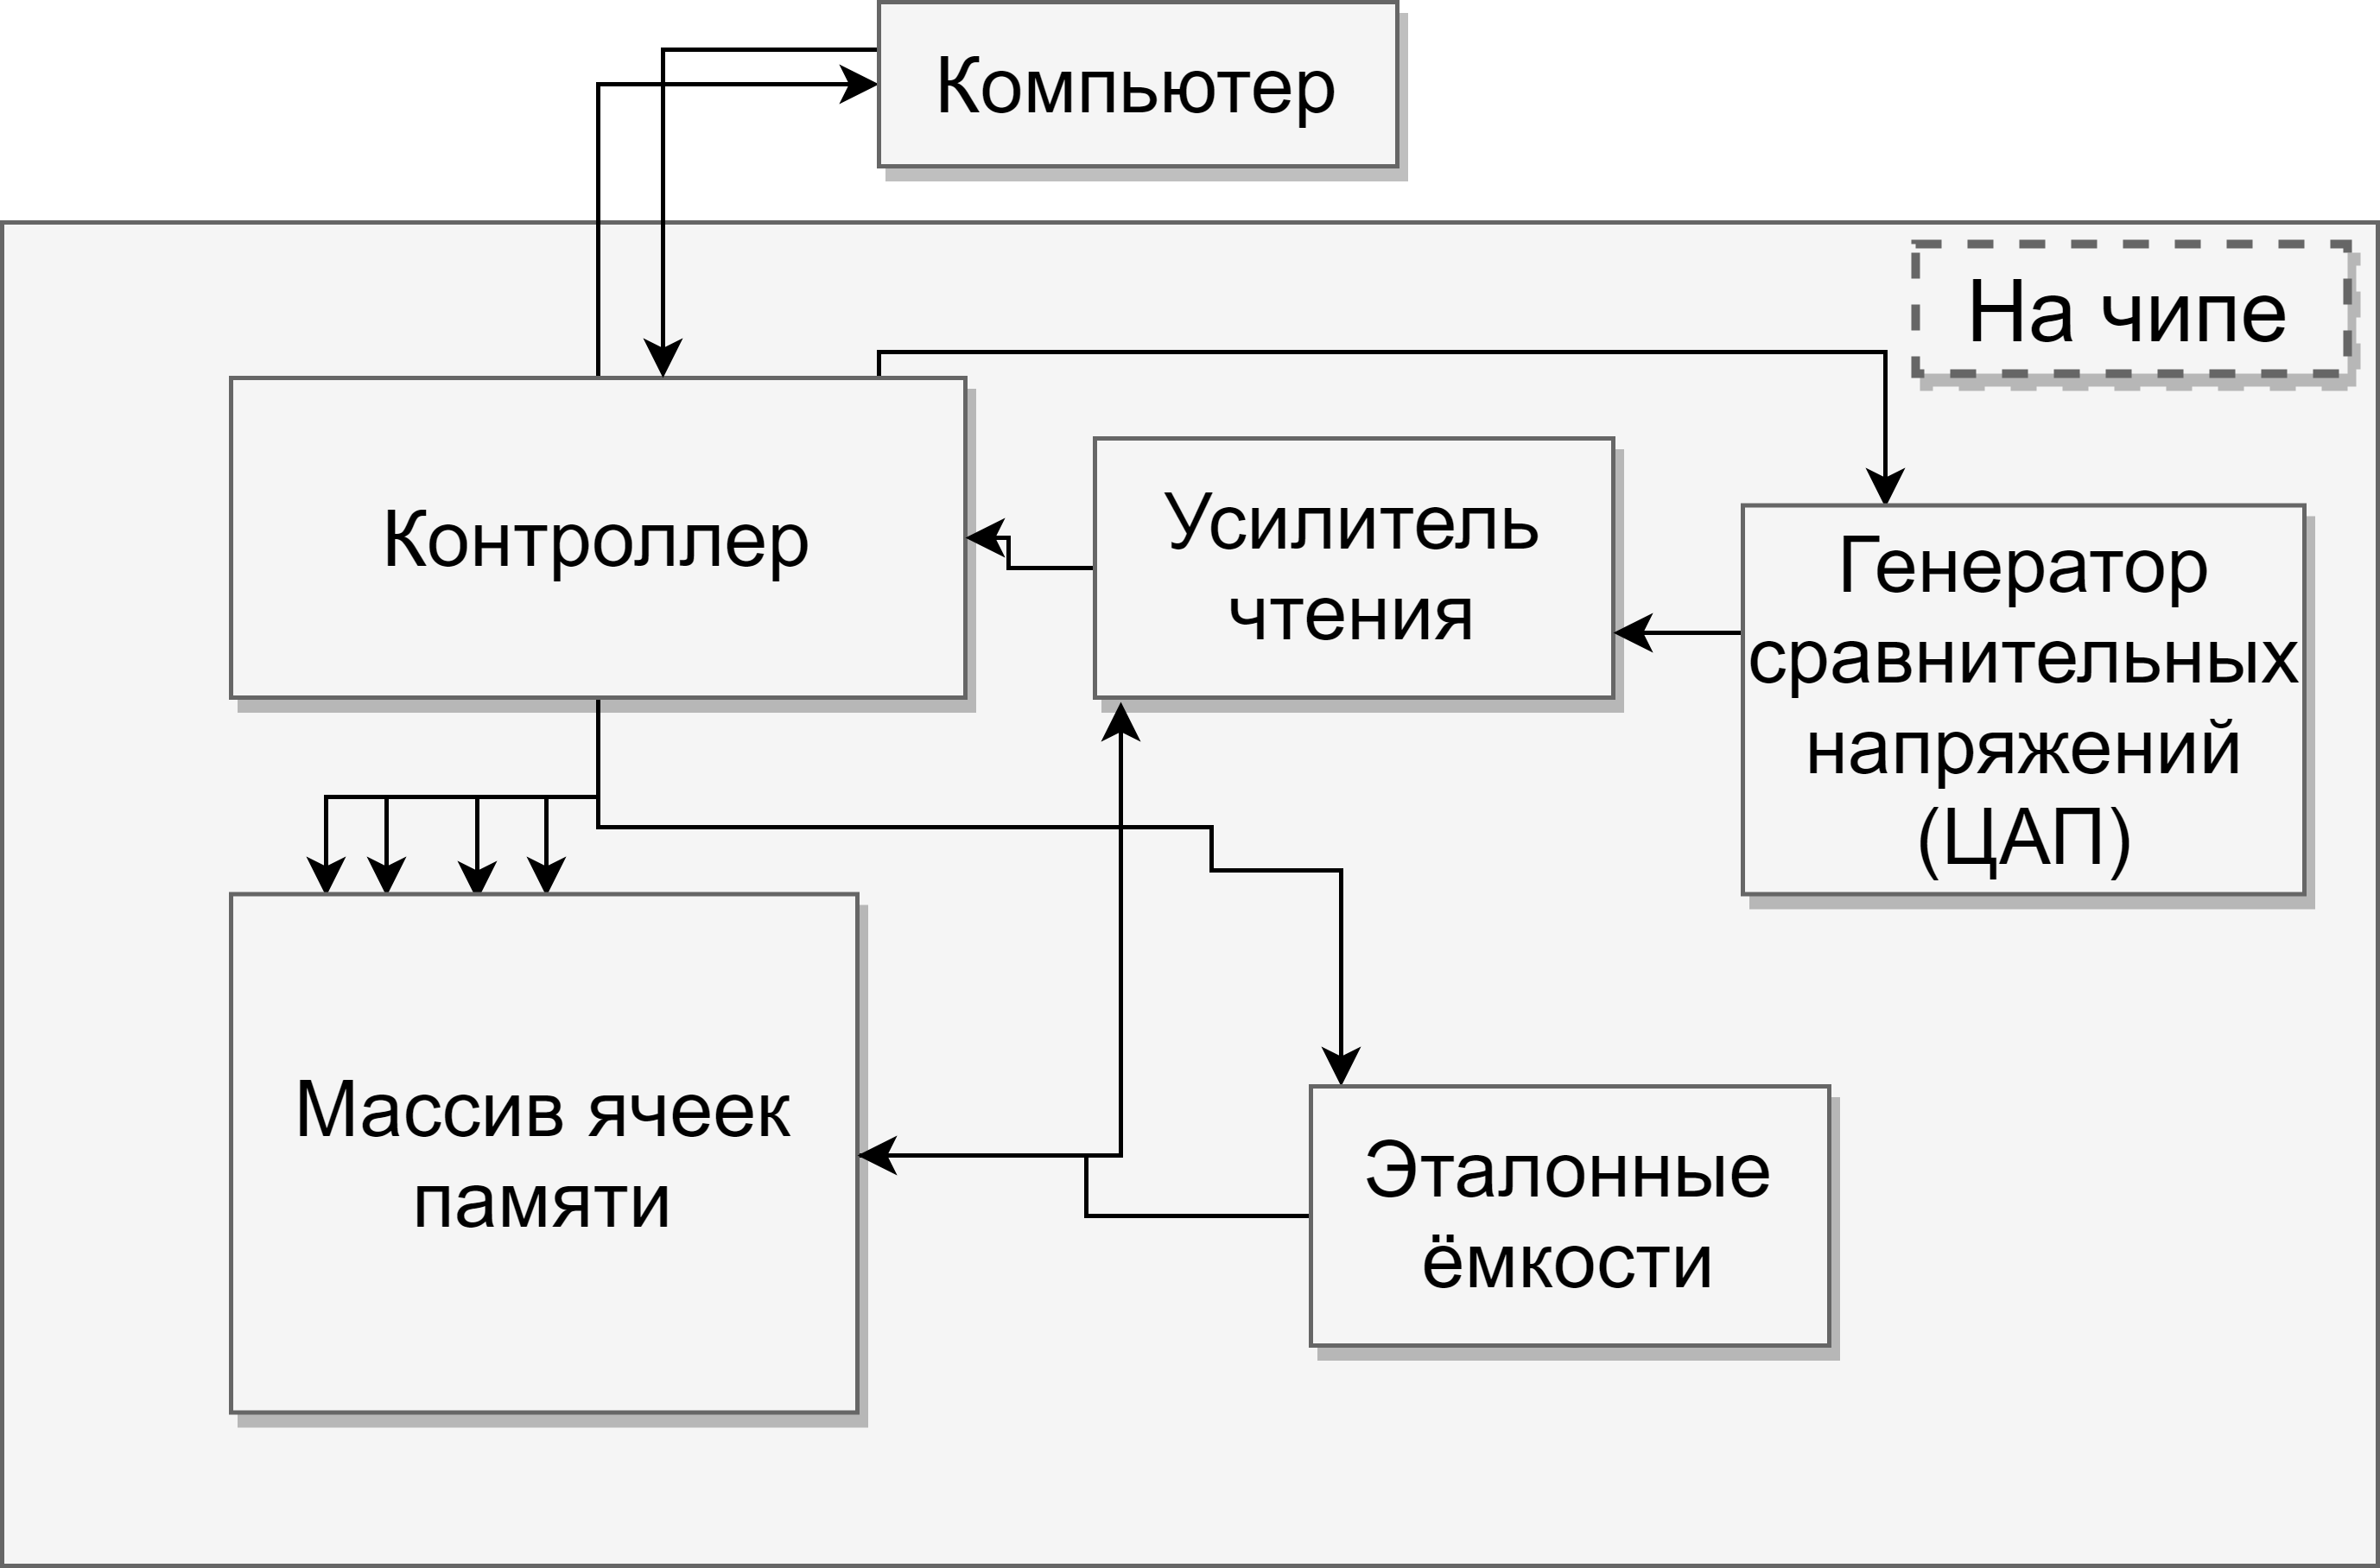
\includegraphics[width=0.6\textwidth]{Scematic.png}\
\end{figure}
Режимы работы устройства:
\begin{enumerate}
\item Стандартные чтение и запись (как память)
\item Измерение остаточной поляризации ячеек (как измерительный прибор)
\item Измерение ёмкости линии битов (как измерительный прибор)
\item Измерение характеристик усилителя 
\end{enumerate}

 \end{center}
}



\frame{\frametitle{Топология ячейки памяти}
\begin{center} 
 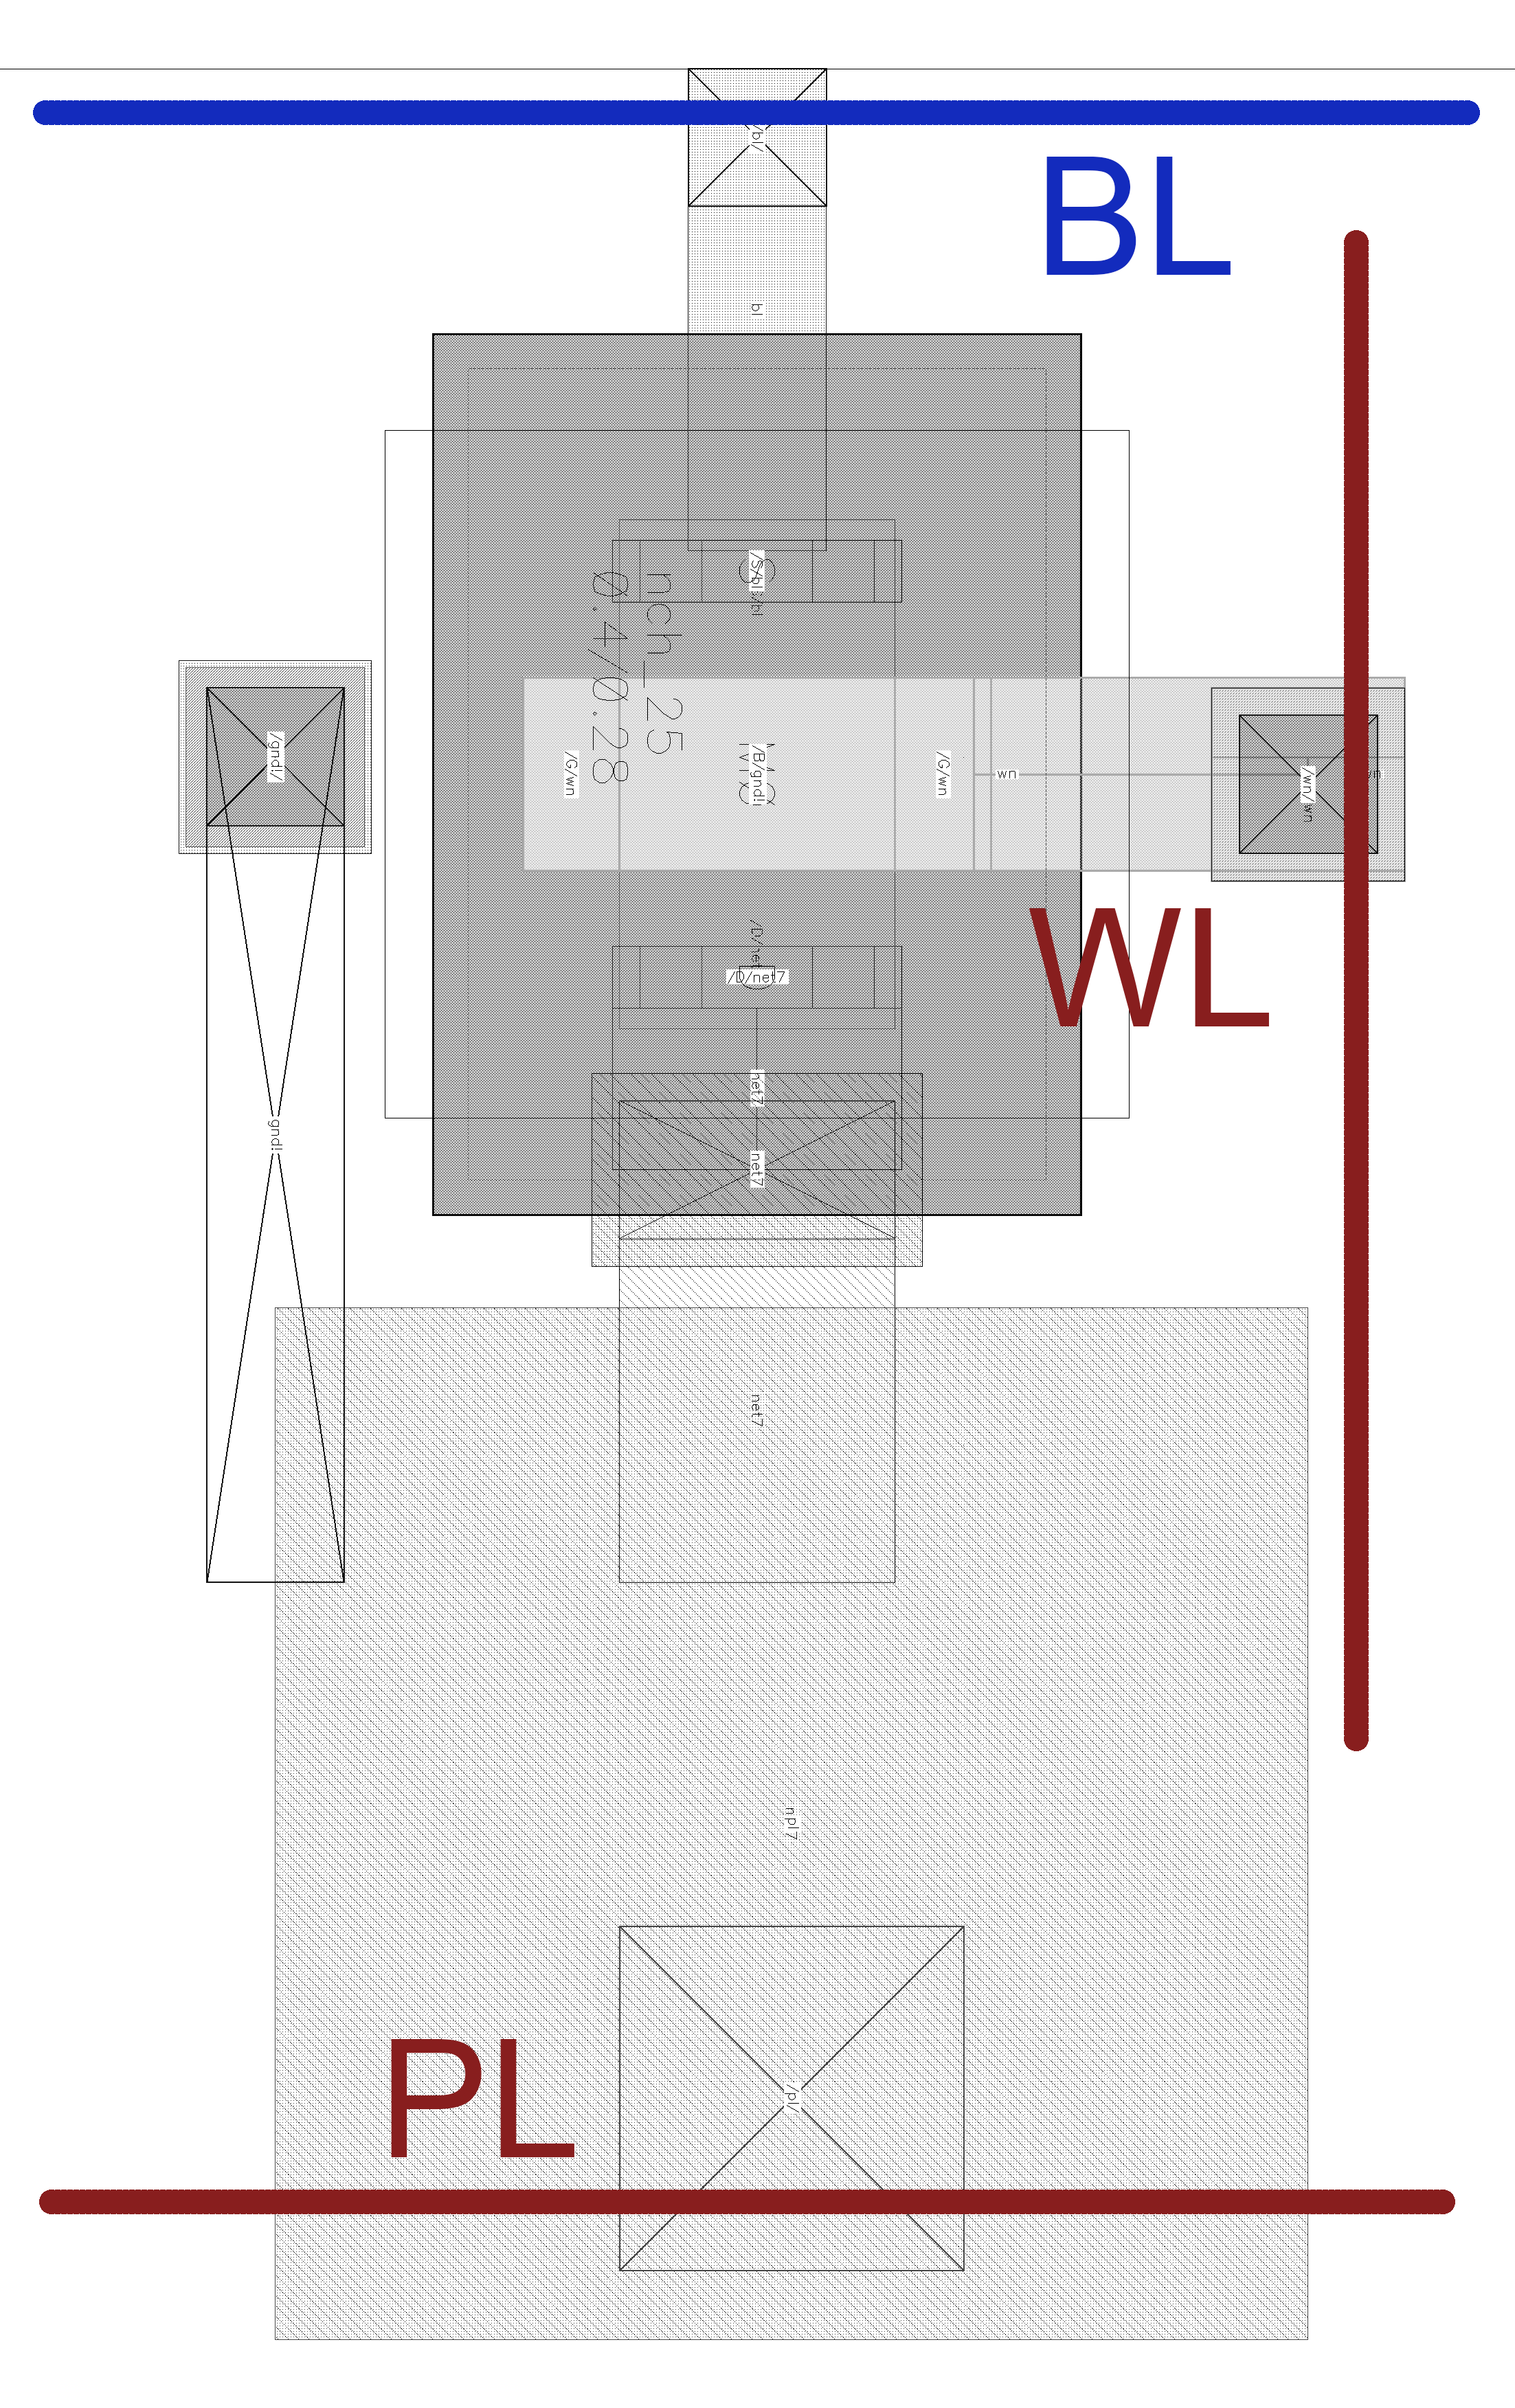
\includegraphics[width=0.4\textwidth]{cell_h.png}
 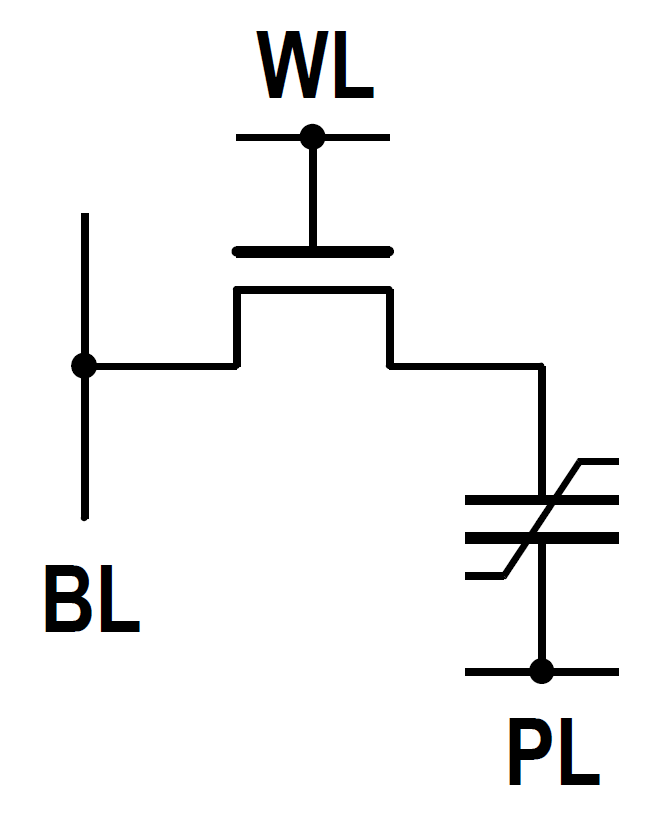
\includegraphics[width=0.4\textwidth]{FRAM-fig1.png}
\end{center}
}


\frame{\frametitle{ Схематика массива памяти}
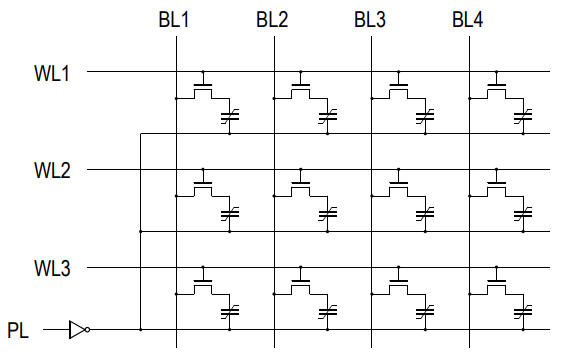
\includegraphics[width=0.5\textwidth]{FRAM_array.png}
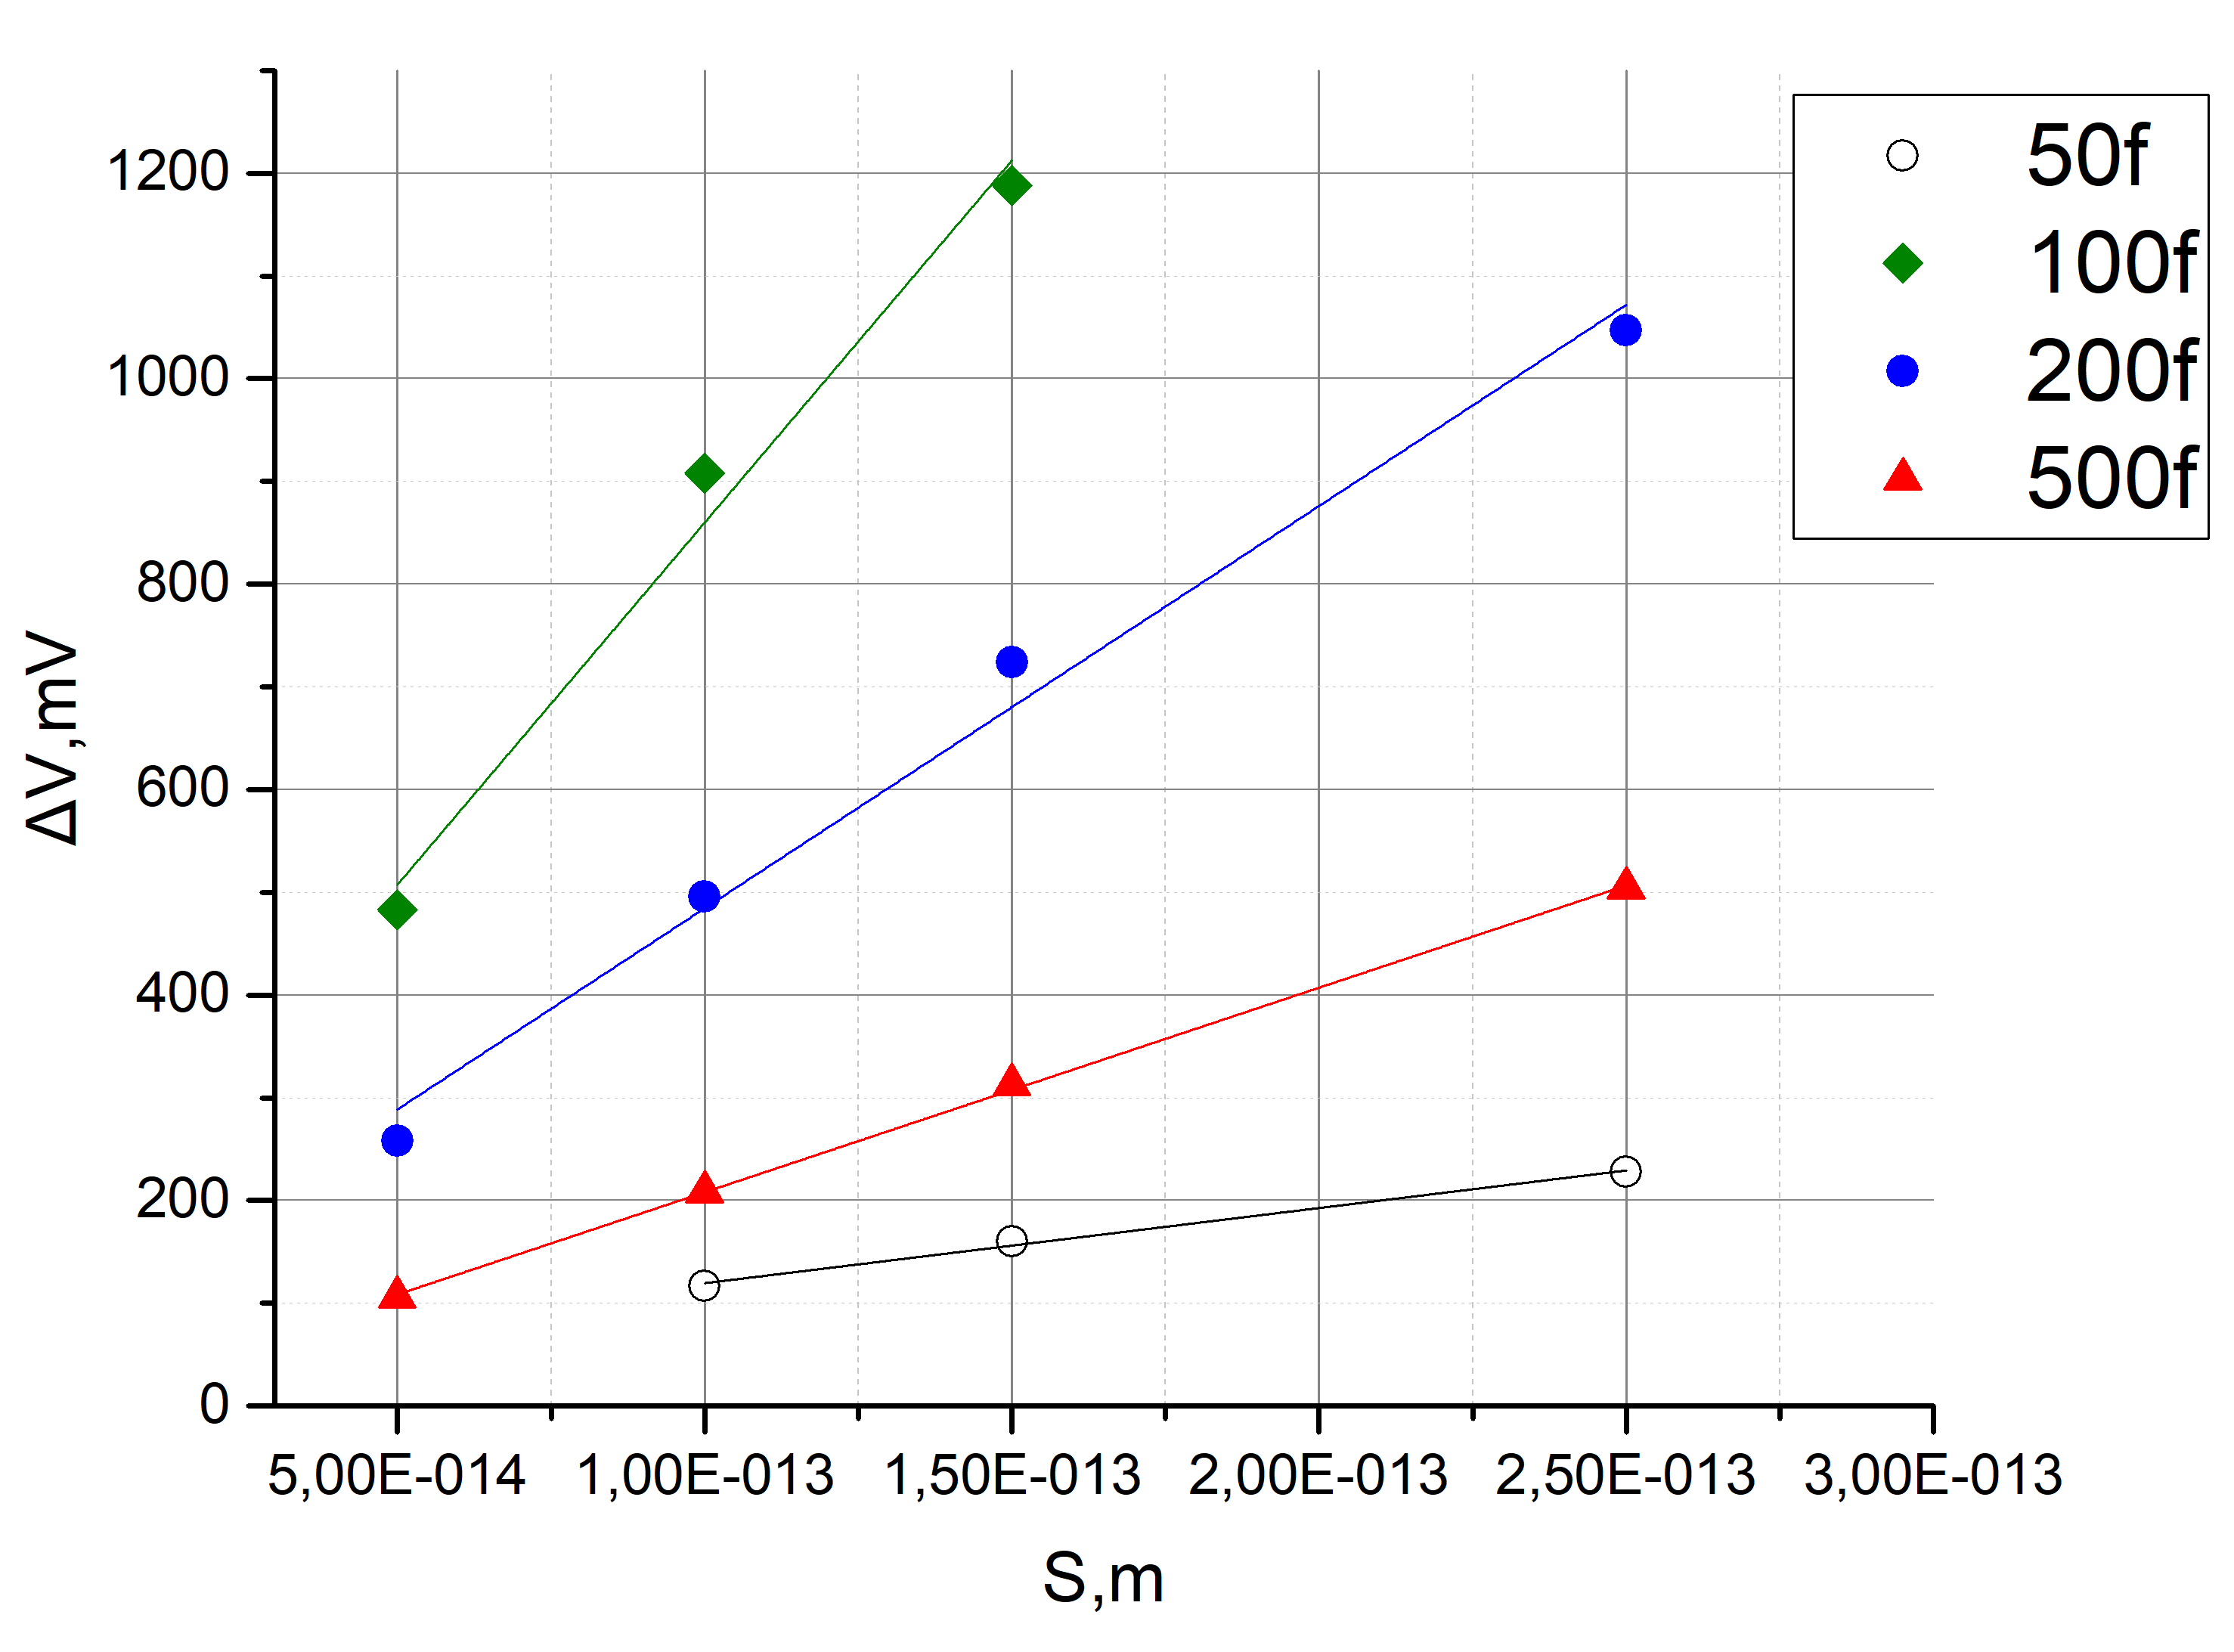
\includegraphics[width=0.47\textwidth]{c_bl.png}
}










\frame{\frametitle{Конструкция усовершенствованного дифференциального неразрушающего  усилителя чтения }
 \begin{center} 

       \begin{tabular}{cl}  
         \begin{tabular}{c}
            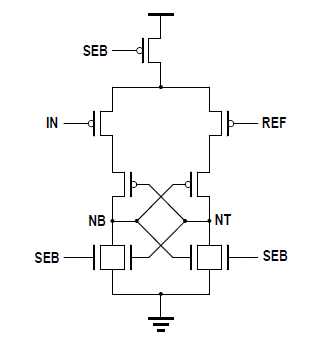
\includegraphics[width=0.5\textwidth]{SA.png}
           \end{tabular}
           & \begin{tabular}{l}
             \parbox{0.4\linewidth}{%  change the parbox width as appropiate
             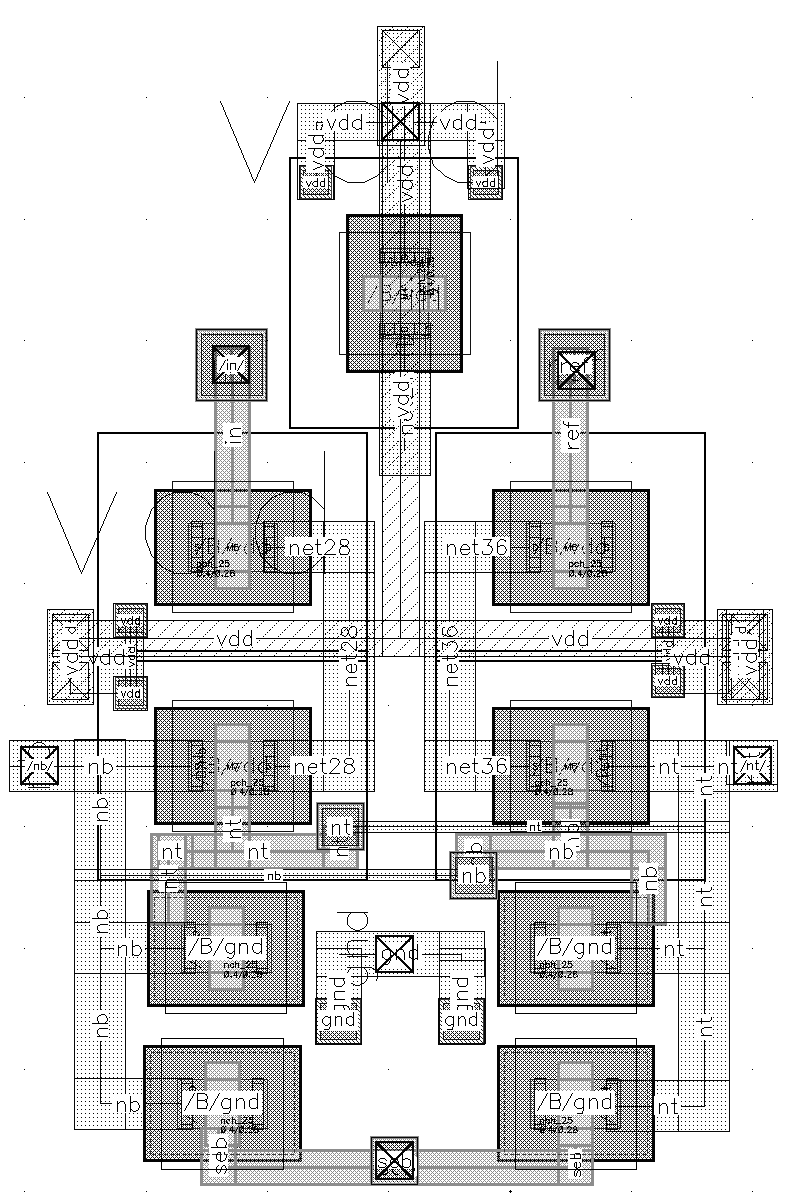
\includegraphics[width=0.4\textwidth]{AMP_v.png}
    }
         \end{tabular}  \\
\end{tabular}
 \end{center}
}







\frame{
 \begin{center} 
  \begin{figure}
 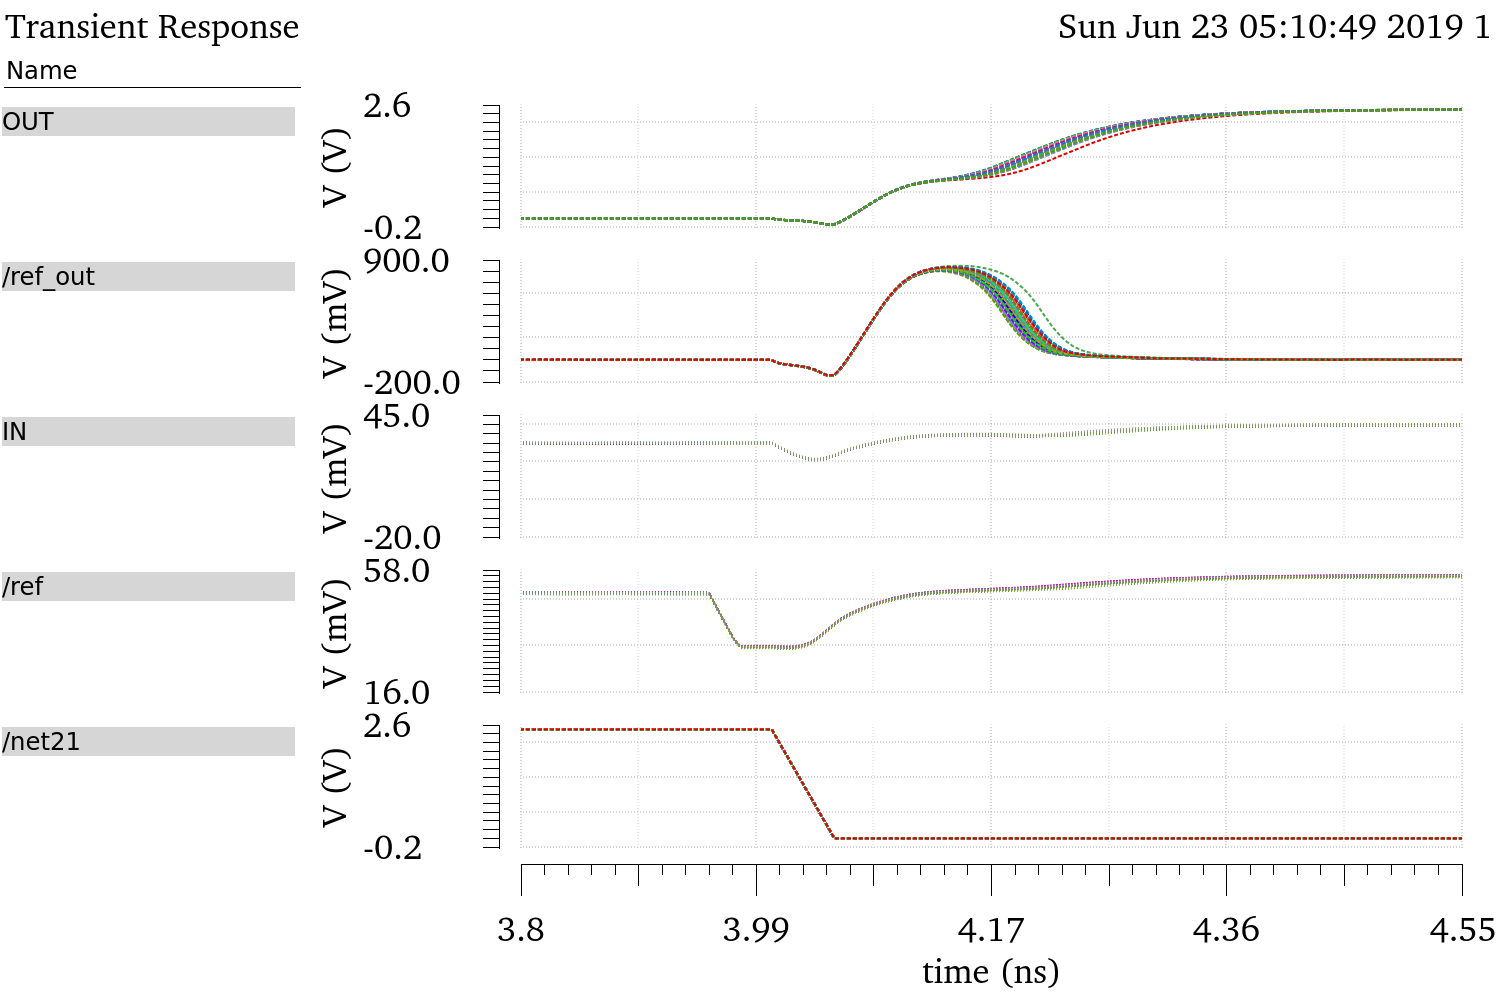
\includegraphics[width=1\textwidth]{ok.png}
 \caption{ Пример успешного сравнения зарядов. Ансамбль из 200 испытаний с учетом полосы шумов по методу Монте Карло в  САПР Cadence Virtuoso . }
 \end{figure}
 \end{center}
}

\frame{
 \begin{center} 
  \begin{figure}
 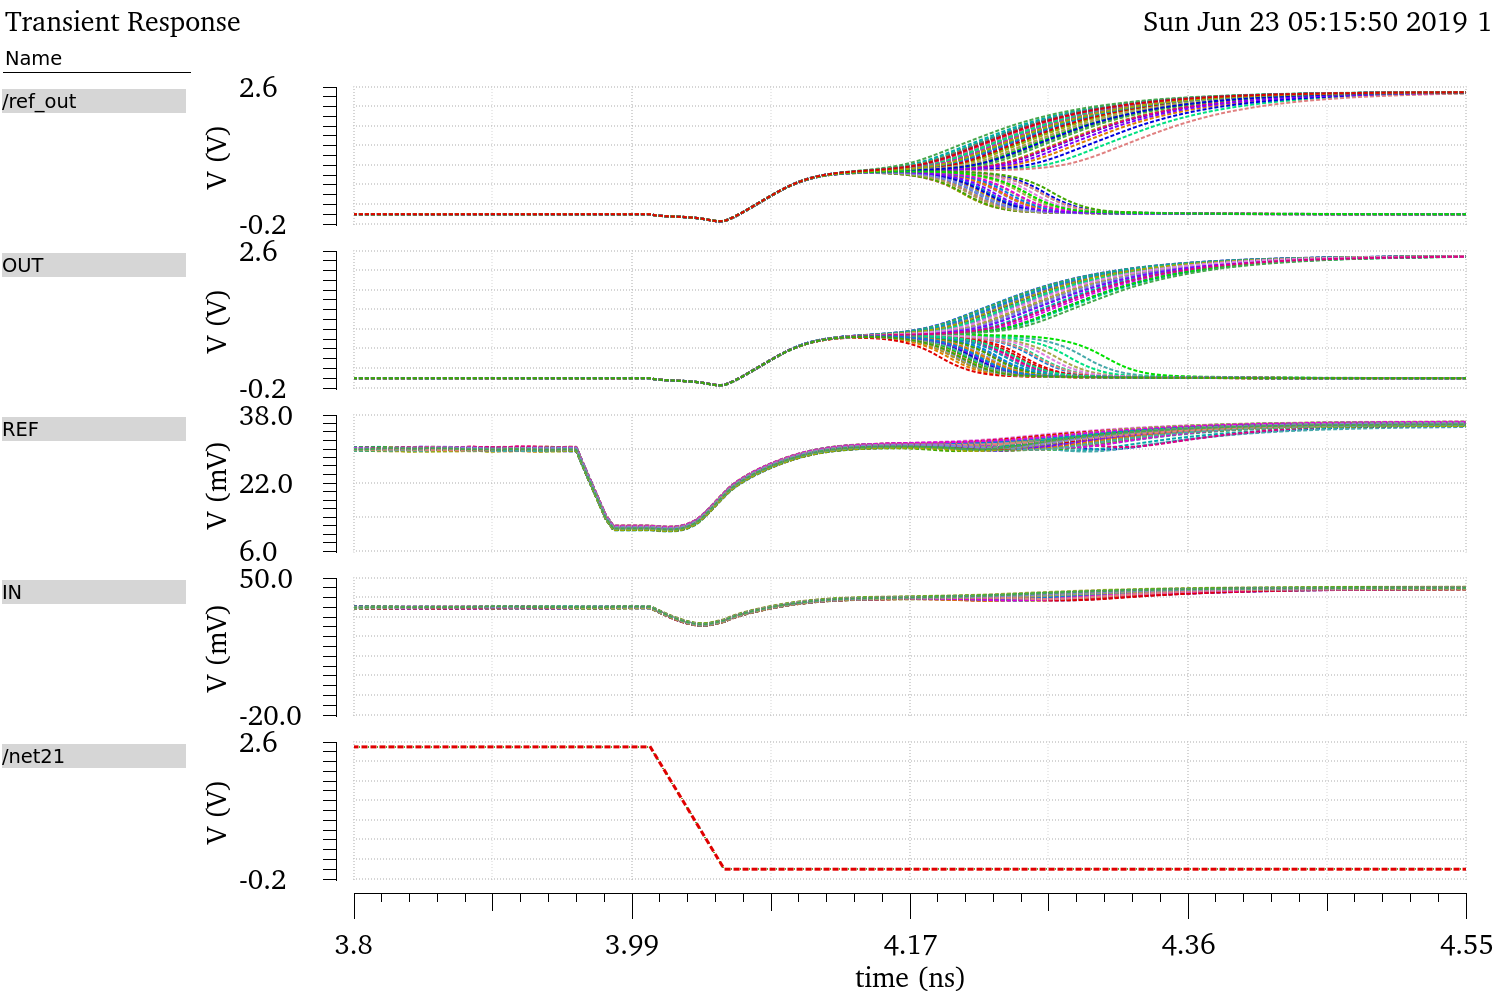
\includegraphics[width=1\textwidth]{fail.png}
 \caption{ Пример невозможности  сравнения из за влияния теплового шума.  Ансамбль из 200 испытаний с учетом полосы шумов по методу Монте Карло в  САПР Cadence Virtuoso. }
 \end{figure}
 \end{center}
}


\frame{
 \begin{center} 
 \begin{figure}
 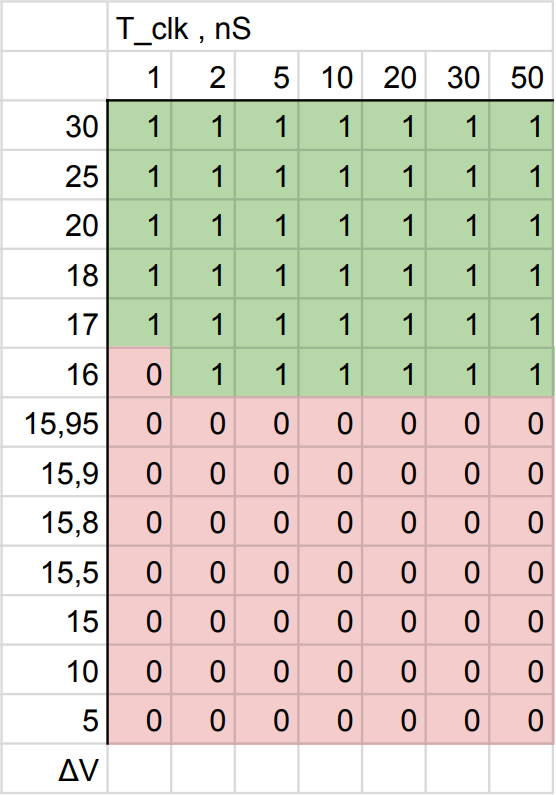
\includegraphics[width=0.45\textwidth]{shmoo.png}
 \caption{Пределы разности сравнения при $V_{ref} = 30mV $ , как видно точность измерения порядка 16 mV, определяется тепловым шумом, на различных частотах ( временная симуляция с учетом полосы шумов по методу Монте Карло в  Cadence Virtuoso)}
 \end{figure}
 \end{center}
}














\frame{\frametitle{Итог:}
 \begin{center}
  \begin{enumerate}
	\item Освоен способ относительно достоверной симуляции сегнетоэлектрического конденсатора при аналоговой спайс симуляции.
	\item Произведена оценка отношения плотности памяти и объема ее ядер для тестового образца ).
	\item Произведена оценка возможности стабильной работы усилителя, а как следственно частотный и габаритный предел создания FRAM на данной технологии.
	\item Создана топология для запуска тестового чипа в производство.
  \end{enumerate} %на самом деле задач было больше, но они не уместились на слайд!
 \end{center}
}





\frame{
 \begin{center} 
 \begin{figure}
 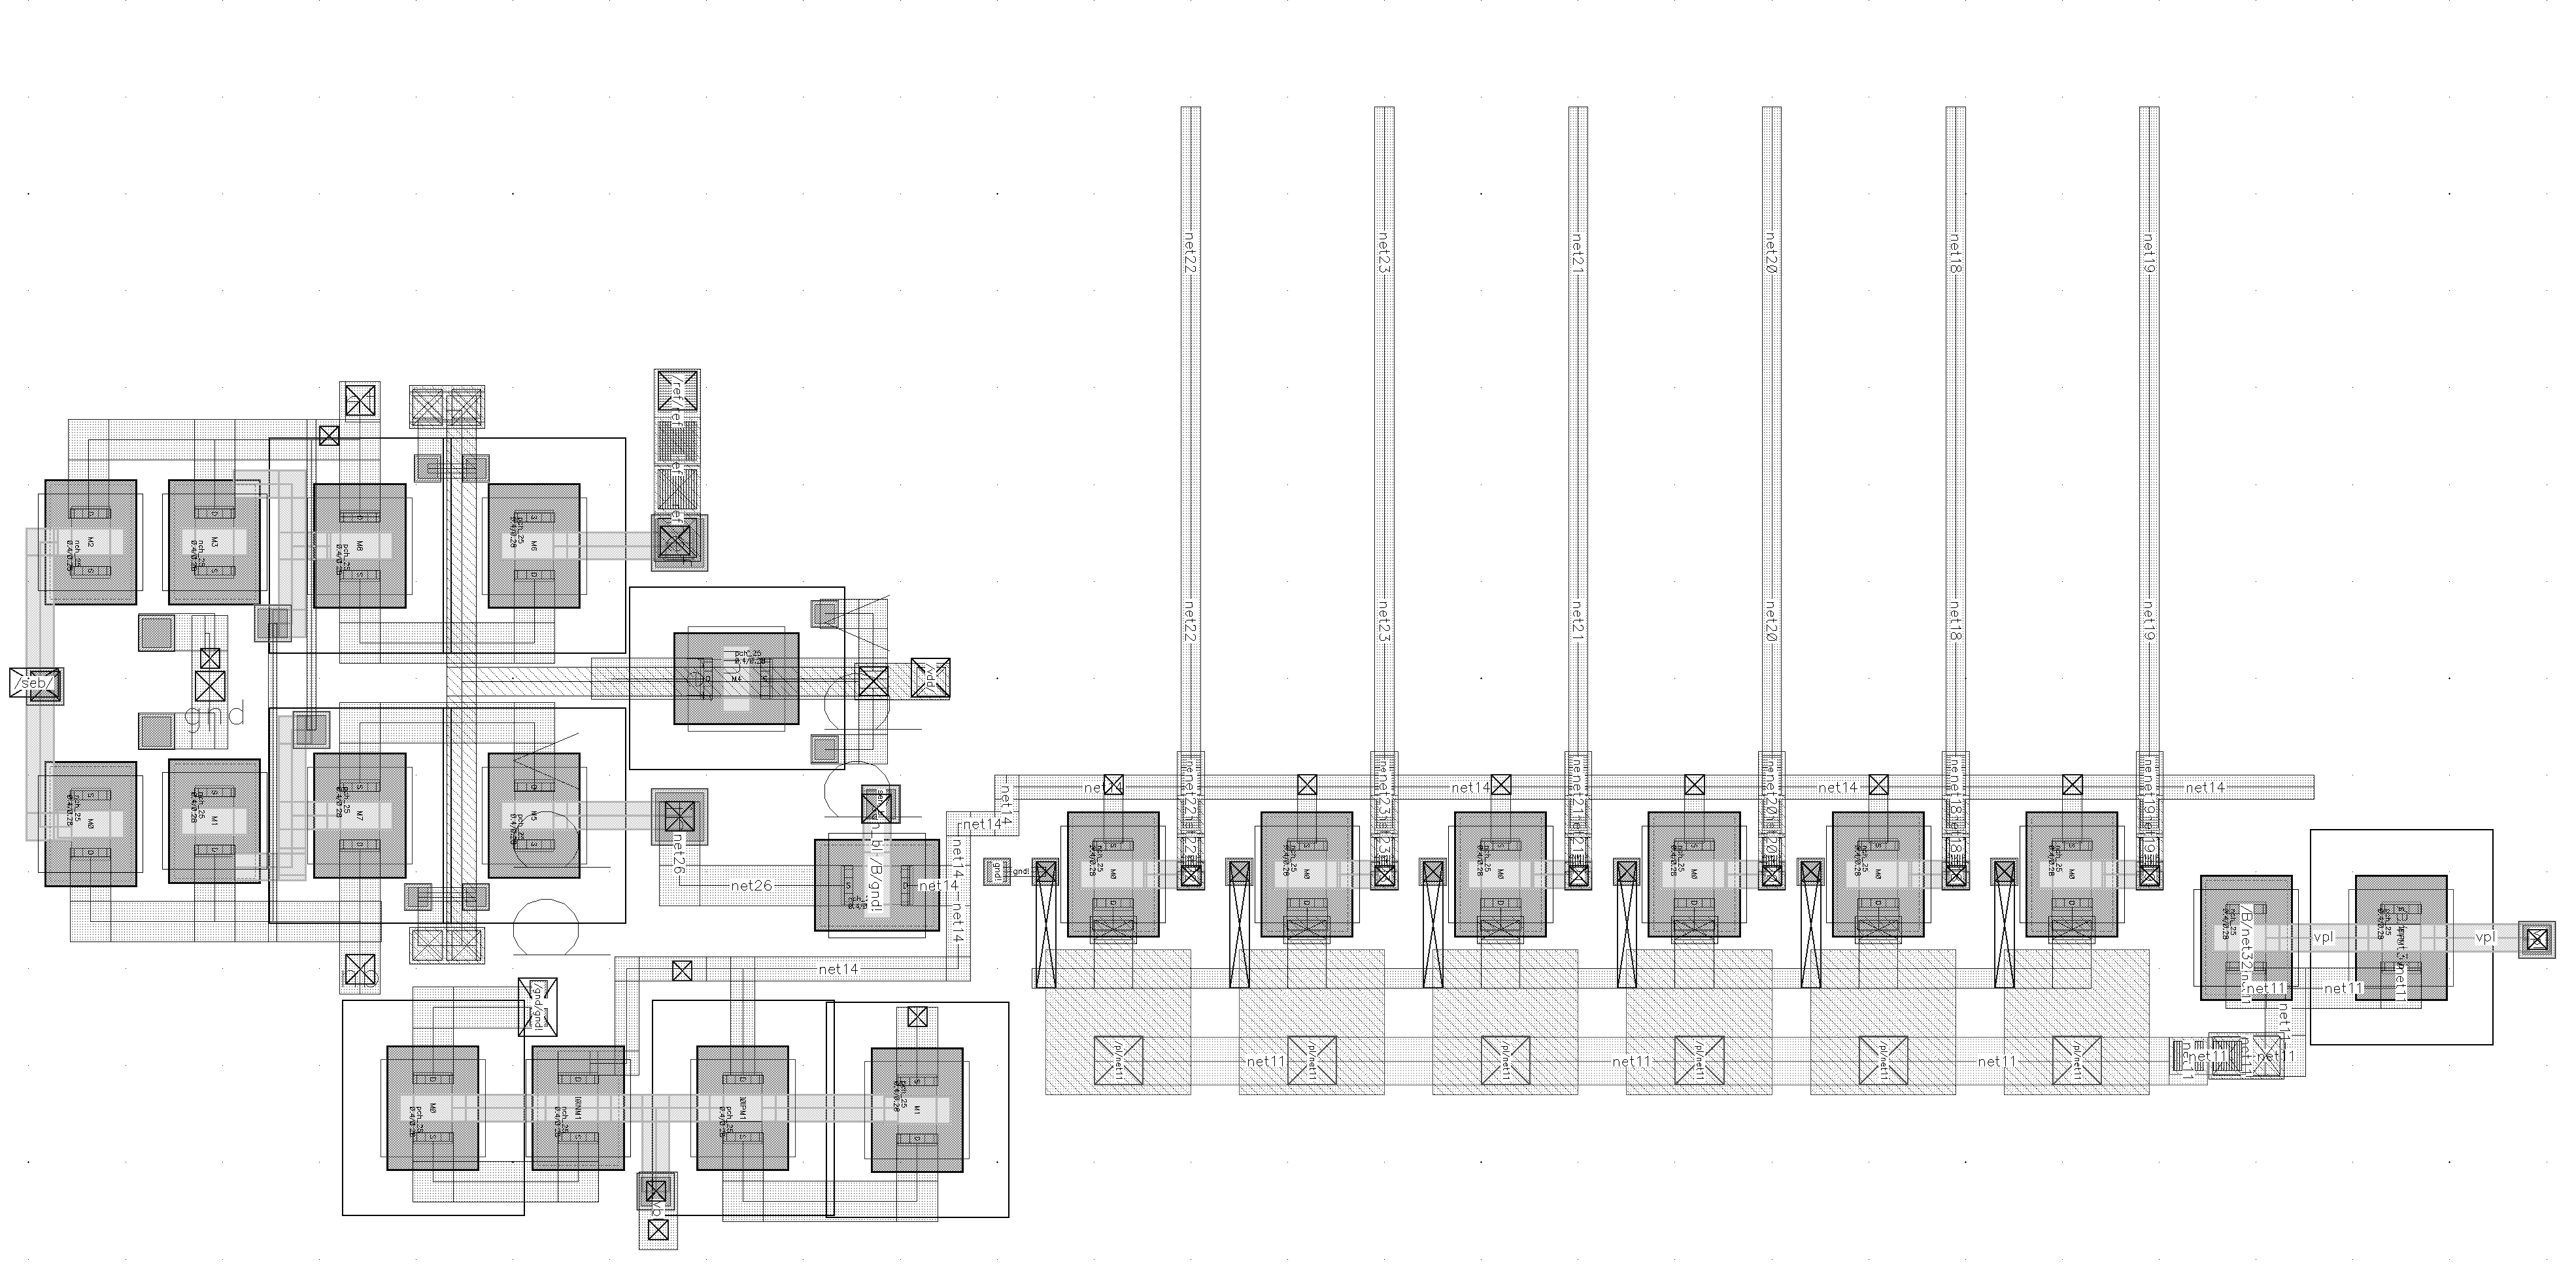
\includegraphics[width=\textwidth]{array_v.png}
 \caption{Топология столбца памяти}
 \end{figure}
 \end{center}
}






\frame{\frametitle{ИСТОЧНИКИ}
 \begin{itemize}
 	\item{\small Mitigating wakeup effect and improving
endurance of ferroelectric $Hf_{0.5}Zr_{0.5}O_2$ thin
films by careful La-doping Published Online: 15 January 2019}
	\item {\small Improved Ferroelectric Switching Endurance of La-Doped $Hf_{0.5}Zr_{0.5}O_2$
Thin Films
Anna G. Chernikova, Maxim G. Kozodaev, Dmitry V. Negrov, Evgeny V. Korostylev,
Min Hyuk Park, Uwe Schroeder, Andrey M. Markeev}
   \item {\small Advanced Circuit Design of Gigabit-Density FRAM
Von der Fakultät für Elektrotechnik und Informationstechnik der Rheinisch-Westfälischen Technischen Hochschule Aachen zur Erlangung des akademischen Grades eines Doktors Dissertation}
   \item { \small Physics of ferroelectrics PBLittlewood January 27, 2002 }
	
   
 \end{itemize}
}













\end{document}